\documentclass{article}

% Language setting
% Replace `english' with e.g. `spanish' to change the document language
\usepackage[english]{babel}

% Set page size and margins
% Replace `letterpaper' with `a4paper' for UK/EU standard size
\usepackage[letterpaper,top=2cm,bottom=2cm,left=3cm,right=3cm,marginparwidth=1.75cm]{geometry}

% Useful packages
\usepackage{amsmath}
\usepackage{graphicx}
\graphicspath{ {./figures/} }
\usepackage[colorlinks=true, allcolors=blue]{hyperref}

\title{Combining two results for better sensitivity to new Higgs: HIG-22-007 Physics Briefing}
\author{Briefing prepared by Stephanie Kwan (skwan@princeton.edu)}

\begin{document}
\maketitle

% \begin{abstract}
% Your abstract.
% \end{abstract}

\section{Is there just one Higgs boson? (157 words)}

The Standard Model theory of particle physics summarizes all known particles and their interactions, but it is not a complete picture of the universe as it cannot account for multiple experimental observations. 

For example, the existence of neutrino mass and dark matter are not addressed by the Standard Model. 

Several beyond the Standard Model theories, such as 2HDM+S (two Higgs doublet models extended by a scalar), address these observations by allowing for an extended group of Higgs particles. The Higgs boson with mass 125 GeV, 
discovered in 2012 by the ATLAS and CMS experiments, would be one of the Higgs particles in this extended group. 

How would we go about searching for these predicted Higgs particles? In one scenario, the 125 GeV Higgs boson can decay to two new intermediate Higgs particles (called ``a" here),
which both decay to known Standard Model particles. If we observe a statistically significant difference between our expected and observed number of events in our ``signal region", i.e. where the measured particles have 
energies and kinematic properties similar to our signal, then we may have evidence of these new particles. 


\section{What did each analysis do, and how do we combine two analyses? (412 words)}

One analysis group studied the case where one ``a" particle decays into two bottom quarks, and the other ``a" decays into two tau leptons, written h $\rightarrow aa \rightarrow 2b2\tau$.
The second analysis group considered the case where one ``a" decays into two bottom quarks, and the other ``a" decays into two muons, i.e. h $\rightarrow aa \rightarrow 2b2\mu$. 

The analyses differ in the muons and taus in their final states, and these particles are extremely different: muons are stable in the detector and are fairly well-reconstructed. 
In comparison, the tau lepton is unstable and decays inside the detector. About 35\% of the time, a tau lepton decays into the lighter leptons (i.e. electrons and muons), and the remaining 65\% of the time, it decays into hadrons, 
which further decay. These possibilities complicate tau reconstruction and distinguishing them from background noise. 

Bottom quarks are heavy enough to decay into jets (showers of particles in a cone), which are also challenging to reconstruct, and difficult to distinguish from low-energy interactions which we are not interested in.

The figure below visualizes a real data event that contains two bottom-quark jets and two tau leptons close together in the detector, which is consistent with the h $\rightarrow aa \rightarrow 2b2\tau$ signature of interest.

\begin{figure}[h]
    \centering
    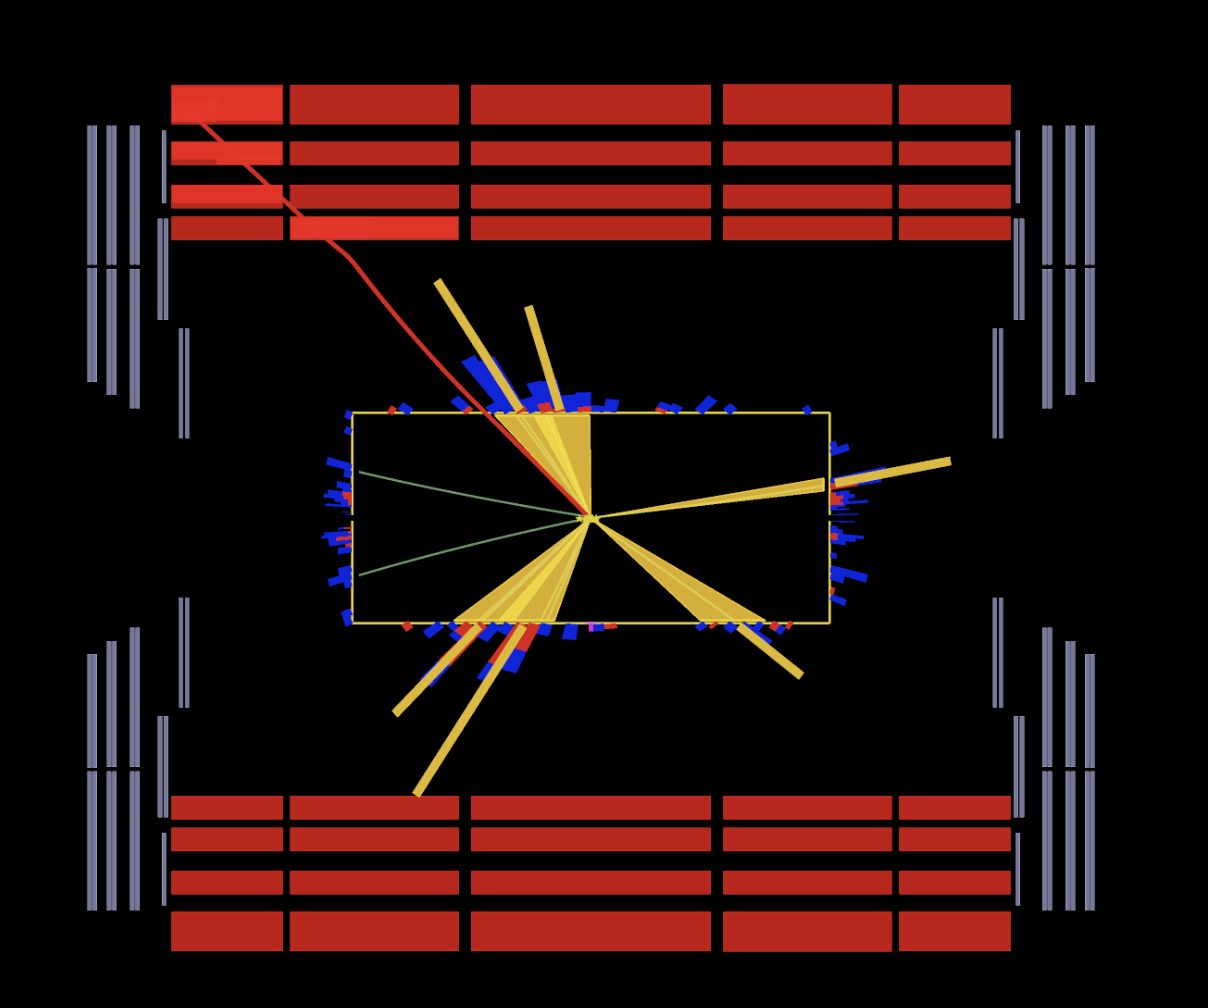
\includegraphics[width=8cm]{fireworks_event1/event1_barrel_slice.png}
    \caption{A data event from 2018 which has a similar signature as the theorized decay of a 125 GeV Higgs boson to two intermediate ``a'' particles, where one decays to two bottom-quark jets (all jets are shown in yellow), 
    and the other decays to two tau leptons. As tau leptons are unstable in the detector, in this event, one tau lepton decays into a muon (muon track in red, connecting to the muon energy deposits shown in red squares).
    The other tau lepton decays into hadrons and produces a jet.
    The blue hits are energy deposits in the hadronic calorimeter (HCAL). The red hits are deposits in the electromagnetic calorimeter (ECAL) respectively.}
\end{figure}




In order to optimize sensitivity to new physics, the two groups independently developed very different strategies.

For instance, the h $\rightarrow aa \rightarrow 2b 2\tau$ group trained a machine learning algorithm to identify signal-like events and reject background events. When applied to real data, the algorithm assigns a score from 0 to 1, 
based on how signal-like the data event is. We use this score to categorize real data based into signal regions (where we expect to see the most signal) and control regions (which we expect to see only background). 

In contrast, the h $\rightarrow aa \rightarrow 2b 2\mu$ group distinguished signal-like events from background events by defining a physical variable based on the masses of the two b quarks and two muons, which tends to be very small for signal-like events,
and large for background events. The advantage of this approach is to utilize the excellent muon mass reconstruction provided by the CMS detector. 

Despite these two different approaches, both analyses are looking for an excess of events as a function of the total mass of the pseudoscalars. 

This allows us to combine our results, improving the experiment's overall sensitivity to the exotic Higgs decay, compared to if the two groups' results were only considered individually. 

\section{How do we interpret our results?}

If our measurements agree well with predictions of the Standard Model within uncertainties, we can ``rule out", or exclude, hypotheses of new physics. We do this by setting exclusion limits.

The exclusion limits for one of the theory types studied (namely, 2HDM+S type 1) are summarized in the plot below, for each individual analysis and the two analyses combined: 


    \begin{figure}[h]
        \centering
        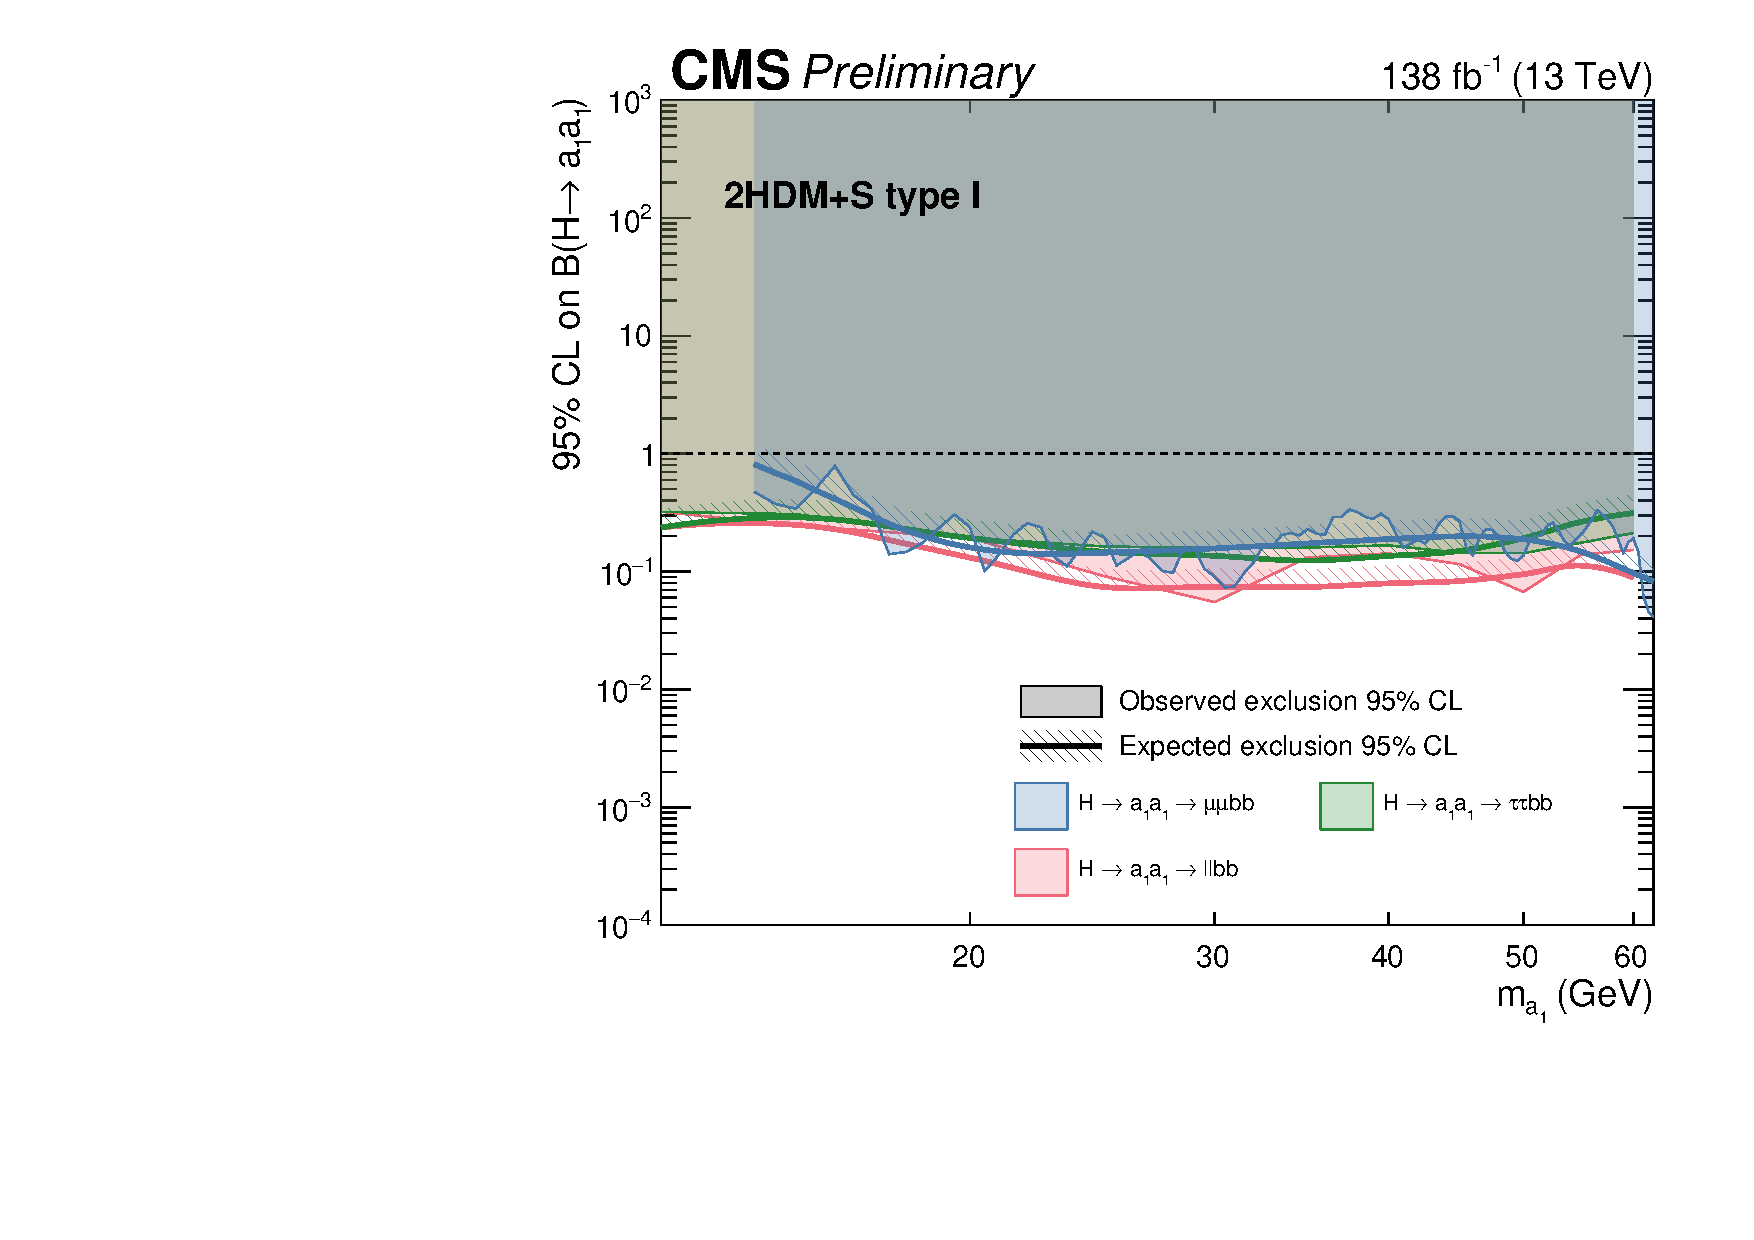
\includegraphics[width=8cm]{full_run2_plot_BRaa_Type1.pdf}
        \caption{Expected and observed limits for 2HDM+S Type I models, for h $\rightarrow aa \rightarrow 2b2\mu$ and h $\rightarrow aa \rightarrow 2b2\tau$ separately, then combined (h $\rightarrow bb \rightarrow \ell\ell$).}
    \end{figure}

The vertical axis is the probability that the 125 GeV Higgs particle decays into two ``a" particles, termed the ``branching ratio'' (B). This cannot be greater than 100\% (the dashed horizontal line). 

The horizontal axis is the mass of the ``a" particle in this theory type, ranging from 10 GeV to 62.5 GeV. 

Since we cannot measure the ``true" decay probability (branching ratio) of H $\rightarrow aa$, instead we set a lower bound, which should be less than the ``true" value 95\% of the time if we were to repeat the measurement over and over again.

This lower bound is calculated for each possible mass of the ``a" particle in each theory, first without fitting to the signal region of the data (giving the ``expected" limits), then with the signal region included (the ``observed" limit). 

If our observed limit is greater than the expected limit with statistical uncertainty (i.e. the solid shaded area falls above the bold line with dashed shaded area), this would be a sign of
disagreement with the Standard Model. However, since our observed limits fall within the expected limits (including uncertainties), our observations are consistent with the Standard Model. 


\section{What does this mean for the big picture?}

By using the full Run 2 dataset from the years 2016 through 2018, and a host of new and improved optimizations, the two analyses were able to set stronger limits than the analyses which used only data from 2016.

Furthermore, combining two measurements provides stronger limits on new hypotheses compared to considering each measurement alone.

These latest results complement and strengthen efforts at the CMS experiment to use the 125 GeV Higgs boson as a probe for searching for signals of new physics. 



\section{References and links}

\begin{itemize}
    \item Exclusion limit figure from \begin{verbatim}https://pdas.web.cern.ch/pdas/HAA/llbb/full_run2_plot_BRaa_Type1.pdf\end{verbatim}
\end{itemize}
\end{document}